% For each digit length L
\subsubsection{ Warping }

% For each index in 1, 2, 3, and carry in 0,1
    For each $i = 1, 2, 3$, $u \in \{0, 1\}^l$, and each $\inc \in \{ {\tt increment, copy } \}$
    % (note: since this might not be the correct notation, in words: do this for each binary encoded digit of length $l$,
    % for each digit-region index, and both copy/increment signals)


    \begin{itemize}
        \item {\prewarp}
            \begin{itemize}

            \item if $u$ ends with 00:
            Create
            $\begin{aligned}[t]
                \prewarp(& \left\langle {\tt PreWarp},   i, u, \inc \right\rangle,
                           \left\langle {\tt FirstWarp}, i, u, \inc \right\rangle \;)
            \end{aligned}$ \\ from the general gadget in Figure~\ref{fig:pre_warp_general}

            \item if $u$ ends with 01:
            Create
            $\begin{aligned}[t]
                \prewarp(& \left\langle {\tt PreWarp},   i, u, \inc \right\rangle,
                           \left\langle {\tt FirstWarp}, i, u, \inc, {\tt msr} \right\rangle \;)
            \end{aligned}$ \\ from the general gadget in Figure~\ref{fig:pre_warp_case2_digit1_msr}

            \item if $u$ ends with 11:
            Create
            $\begin{aligned}[t]
                \prewarp(& \left\langle {\tt PreWarp},   i, u, \inc \right\rangle,
                           \left\langle {\tt FirstWarp}, i, u, \inc, {\tt msr}, {\tt msd} \right\rangle \;)
            \end{aligned}$

            Depending on the number of digits in the MSR, the gadget created in this step will differ.
            If $i$ is 1 (case 1) use the general gadget in Figure~\ref{fig:pre_warp_case1_digit1_msr}.
            If $i$ is 2 (case 2) use the general gadget in Figure~\ref{fig:pre_warp_case2_digit2_msr}.
            If $i$ is 3 (case 3) use the general gadget in Figure~\ref{fig:pre_warp_general}.
        \end{itemize}
        \vspace{.5cm}

        \begin{figure}[H]
            \begin{subfigure}[t]{0.2\textwidth}
                \centering
                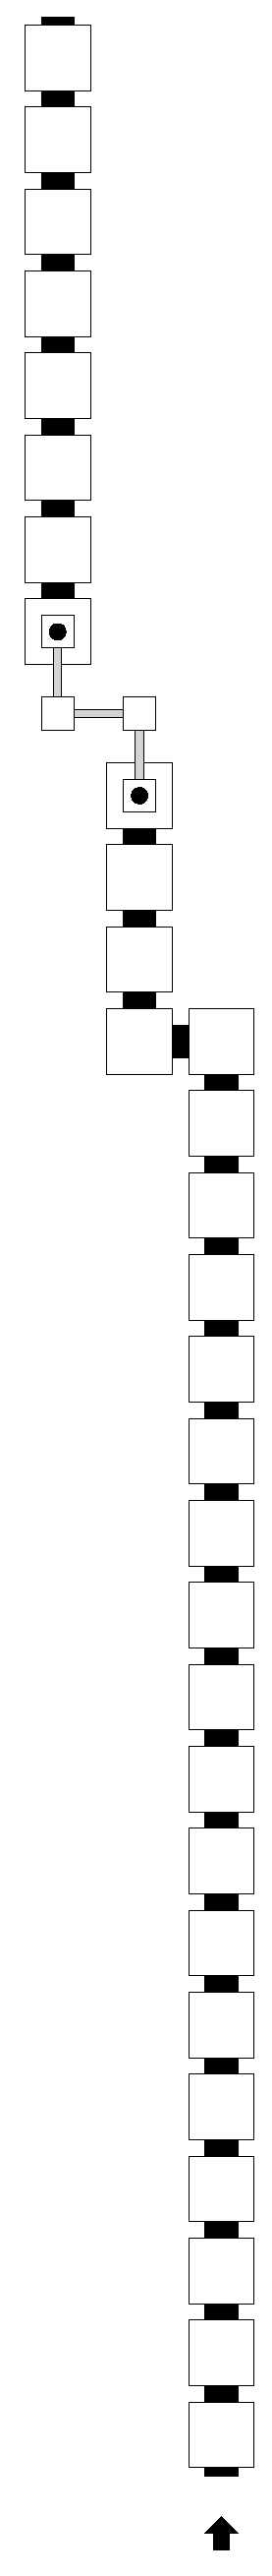
\includegraphics[width=0.2\textwidth]{warping/pre_warp_general}
                \caption{\label{fig:pre_warp_general} General }
            \end{subfigure}%
            ~
            \begin{subfigure}[t]{0.2\textwidth}
                \centering
                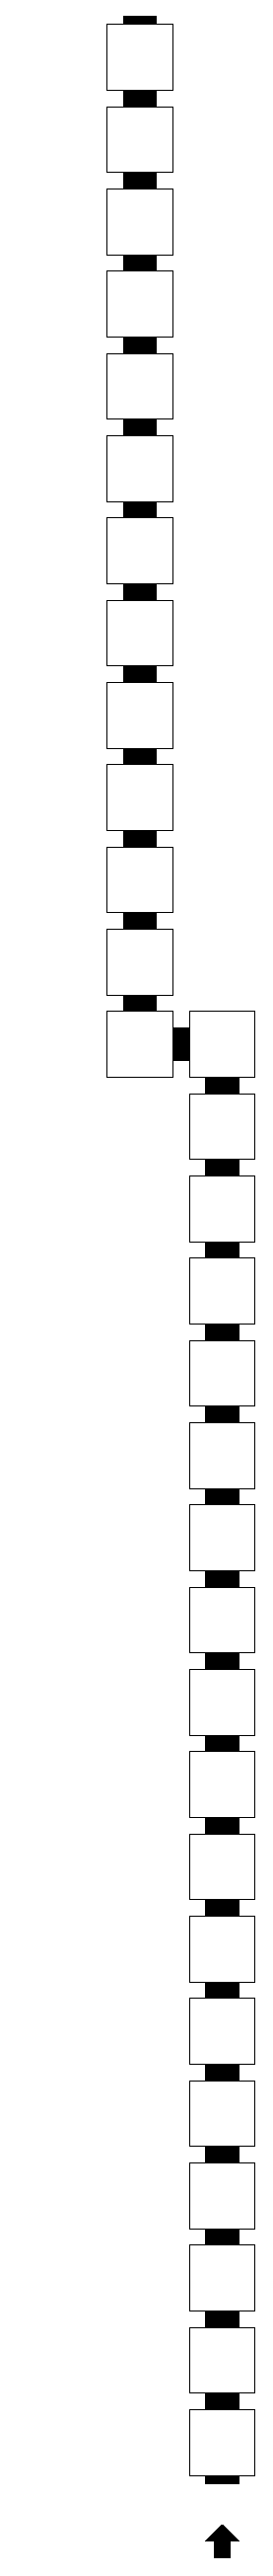
\includegraphics[width=0.2\textwidth]{warping/pre_warp_case1_digit1_msr}
                \caption{\label{fig:pre_warp_case1_digit1_msr} Digit 1 -- Case 1}
            \end{subfigure}%
            ~
            \begin{subfigure}[t]{0.2\textwidth}
                \centering
                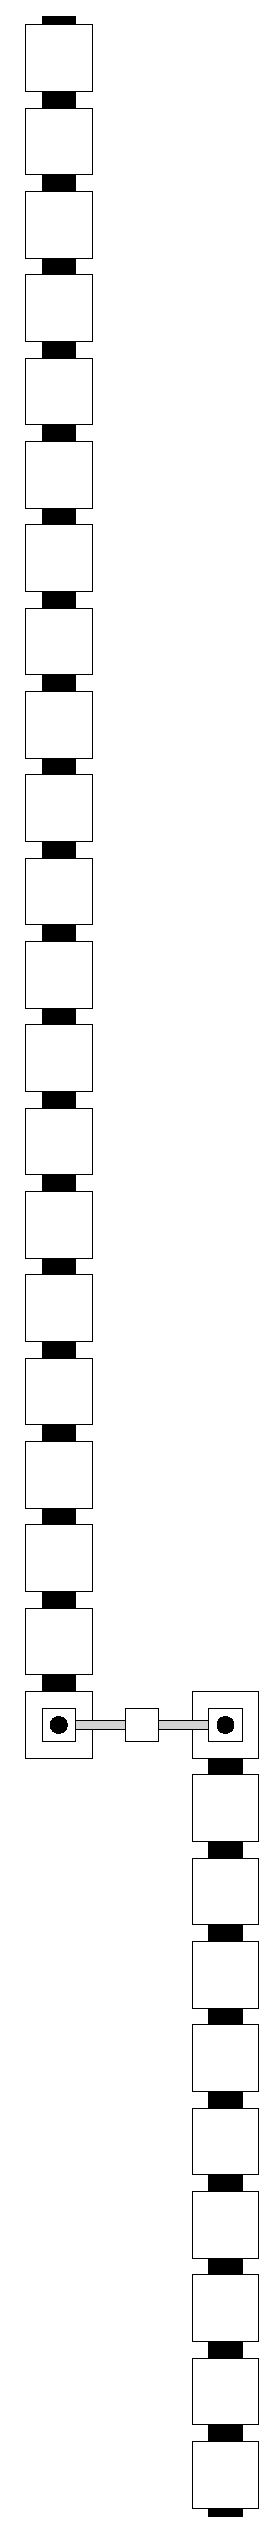
\includegraphics[width=0.2\textwidth]{warping/pre_warp_case2_digit1_msr}
                \caption{\label{fig:pre_warp_case2_digit1_msr} Digit 1 -- Case 2}
            \end{subfigure}%
            ~
            \begin{subfigure}[t]{0.2\textwidth}
                \centering
                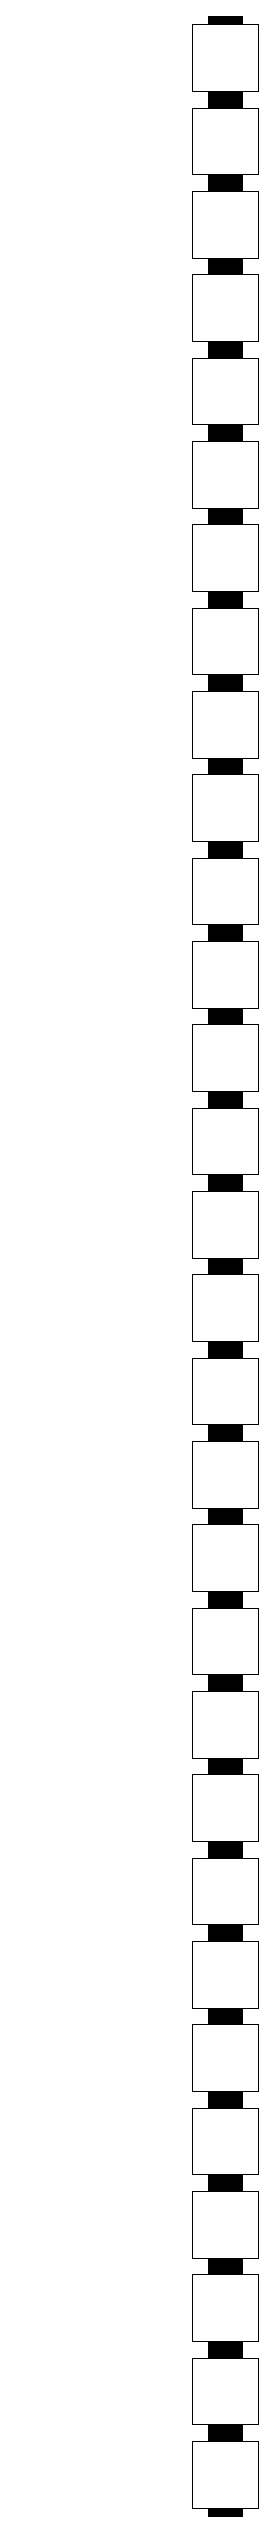
\includegraphics[width=0.2\textwidth]{warping/pre_warp_case2_digit2_msr}
                \caption{\label{fig:pre_warp_case2_digit2_msr} Digit 2 -- Case 2}
            \end{subfigure}%
            ~
            \caption{\label{fig:pre_warp_gadgets} {\prewarp} gadgets }
        \end{figure}


        \item {\firstwarp}: A {\firstwarp} connects to a {\warpbridge} gadget in all cases except when it's assembling
              in the MSR and it is digit 1 in case 1 or 2, in which the {\firstwarp} gadget attaches directly
              to a {\postwarp}.

              \begin{itemize}

                \item Create
                $\begin{aligned}[t]
                    \firstwarp(& \left\langle {\tt FirstWarp},  i, u, \inc \right\rangle, \\
                               & \left\langle {\tt FirstWarp},  i, u, \inc \right\rangle, \\
                               & \left\langle {\tt WarpBridge}, i, u, \inc \right\rangle \;)
                \end{aligned}$
                \vspace{.5cm}

                \item (digit 1, case 2): Create
                $\begin{aligned}[t]
                    \firstwarp(& \left\langle {\tt FirstWarp}, i, u, \inc, {\tt msr} \right\rangle, \\
                               & \left\langle {\tt FirstWarp}, i, u, \inc, {\tt msr} \right\rangle, \\
                               & \left\langle {\tt PostWarp},  i, u, \inc, {\tt msr} \right\rangle \;)
                \end{aligned}$
                \vspace{.5cm}

                \item (digit 1, case 1): Create
                $\begin{aligned}[t]
                    \firstwarp(& \left\langle {\tt FirstWarp}, i, u, \inc, {\tt msr}, {\tt msd} \right\rangle, \\
                               & \left\langle {\tt FirstWarp}, i, u, \inc, {\tt msr}, {\tt msd} \right\rangle, \\
                               & \left\langle {\tt PostWarp},  i, u, \inc, {\tt msr}, {\tt msd} \right\rangle \;)
                \end{aligned}$
                \vspace{.5cm}

                \item (digit 2, case 2): Create
                $\begin{aligned}[t]
                    \firstwarp(& \left\langle {\tt FirstWarp},  i, u, \inc, {\tt msr}, {\tt msd} \right\rangle, \\
                               & \left\langle {\tt FirstWarp},  i, u, \inc, {\tt msr}, {\tt msd} \right\rangle, \\
                               & \left\langle {\tt WarpBridge}, i, u, \inc, {\tt msr}, {\tt msd} \right\rangle \;)
                \end{aligned}$
                \vspace{.5cm}

                \item (digit 3, case 3): Create
                $\begin{aligned}[t]
                    \firstwarp(& \left\langle {\tt FirstWarp},  i, u, \inc, {\tt msr}, {\tt msd} \right\rangle, \\
                               & \left\langle {\tt FirstWarp},  i, u, \inc, {\tt msr}, {\tt msd} \right\rangle, \\
                               & \left\langle {\tt WarpBridge}, i, u, \inc, {\tt msr}, {\tt msd} \right\rangle \;)
                \end{aligned}$
                \vspace{.5cm}

            \end{itemize}
        \vspace{.5cm}

        \item {\warpbridge}: a {\warpbridge} gadget binds the last tile of the {\firstwarp} gadgets to the
             first tile of the {\secondwarp} gadgets. For digit 1 in cases 1 and 2, the
             {\warpbridge} is omitted from the {\warpunit}.

        \begin{itemize}

            \item if $u$ ends with 00:\\
            Create
            $\begin{aligned}[t]
                \warpbridge(& \left\langle {\tt WarpBridge}, i, u, \inc \right\rangle,
                              \left\langle {\tt SecondWarp}, i, u, \inc \right\rangle \;)
            \end{aligned}$ \\ from the general gadget in Figure~\ref{fig:warp_bridge_general}
            \vspace{.5cm}

            \item if $u$ ends with 11 and $i$ is 2: \\
            Create
            $\begin{aligned}[t]
                \warpbridge(& \left\langle {\tt WarpBridge}, i, u, \inc, {\tt msr}, {\tt msd} \right\rangle,
                              \left\langle {\tt SecondWarp}, i, u, \inc, {\tt msr}, {\tt msd} \right\rangle \;)
            \end{aligned}$ \\ from the general gadget in Figure~\ref{fig:warp_bridge_case2_digit2_msr}
            \vspace{.5cm}

            \item if $u$ ends with 11 and $i$ is 3: \\
            Create
            $\begin{aligned}[t]
                \warpbridge(& \left\langle {\tt WarpBridge}, i, u, \inc, {\tt msr}, {\tt msd} \right\rangle,
                              \left\langle {\tt SecondWarp}, i, u, \inc, {\tt msr}, {\tt msd} \right\rangle \;)
            \end{aligned}$ \\ from the general gadget in Figure~\ref{fig:warp_bridge_general}
            \vspace{.5cm}
        \end{itemize}

        \begin{figure}[H]
            \centering
            \begin{subfigure}[t]{0.2\textwidth}
                \centering
                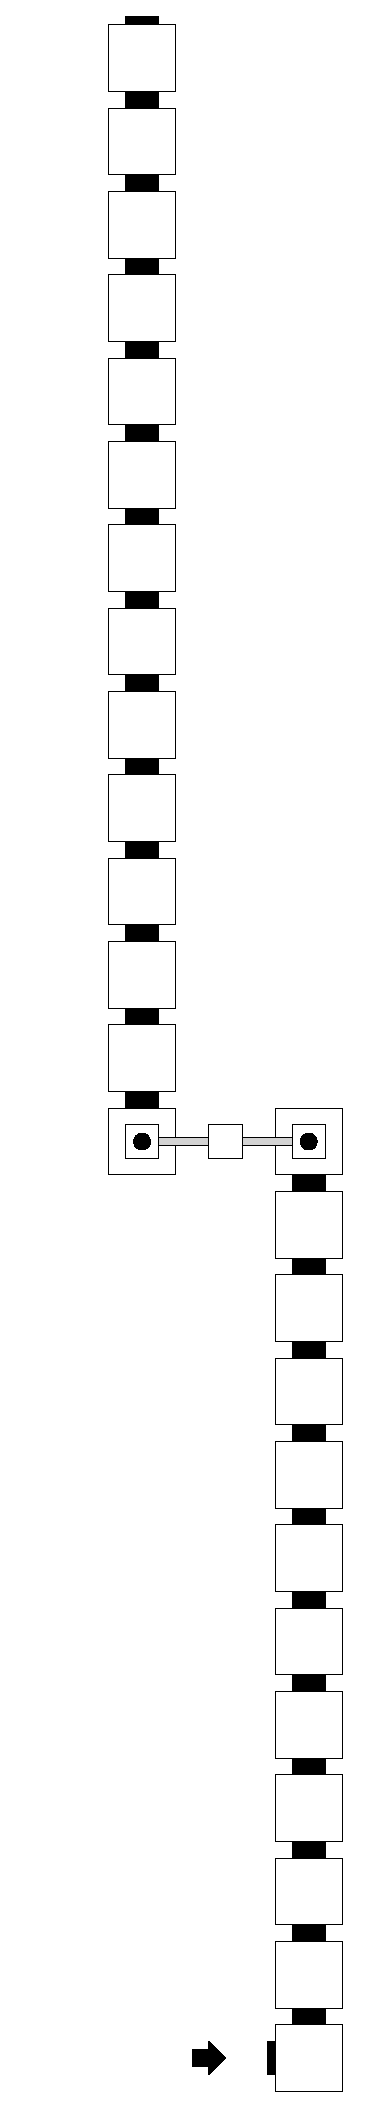
\includegraphics[width=0.2\textwidth]{warping/warp_bridge_general}
                \caption{\label{fig:warp_bridge_general} General}
            \end{subfigure}%
            ~
            \begin{subfigure}[t]{0.2\textwidth}
                \centering
                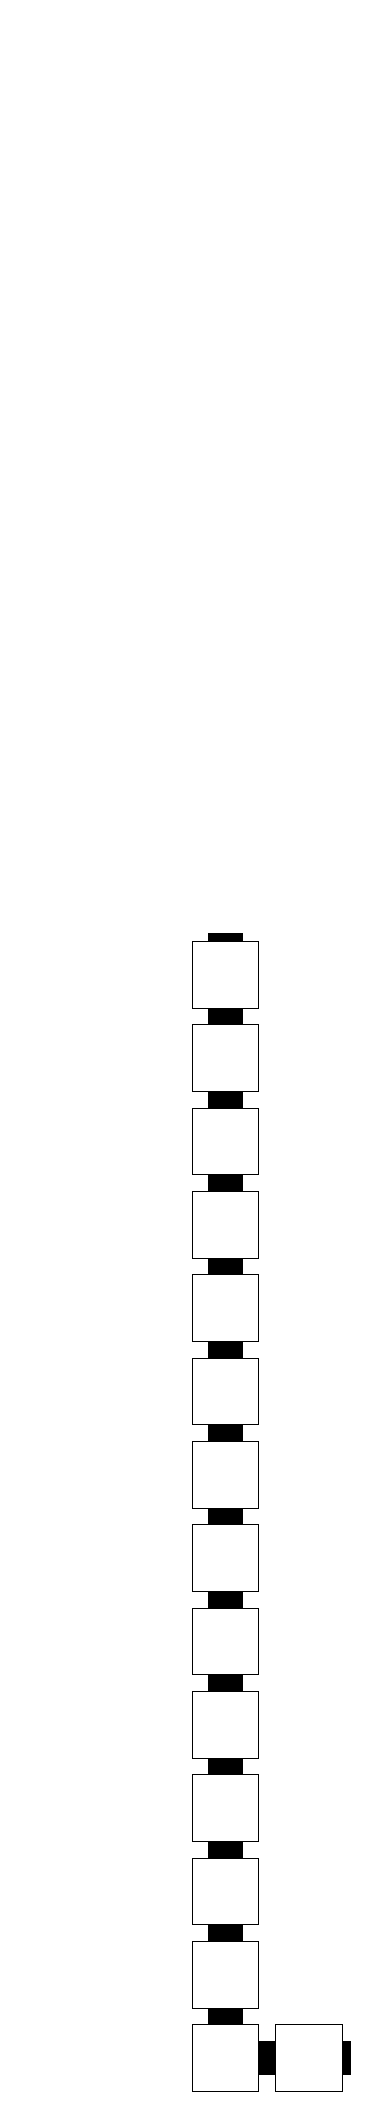
\includegraphics[width=0.2\textwidth]{warping/warp_bridge_case2_digit2_msr}
                \caption{\label{fig:warp_bridge_case2_digit2_msr} Digit 2 -- Case 2}
            \end{subfigure}%
            ~\caption{\label{fig:warp_bridge} {\tt Warp\_Bridge} gadgets}
        \end{figure}


        \item {\secondwarp}:
        \begin{itemize}
        \item Create
        $\begin{aligned}[t]
            \secondwarp(& \left\langle {\tt SecondWarp}, i, u, \inc \right\rangle, \\
                        & \left\langle {\tt SecondWarp}, i, u, \inc \right\rangle, \\
                        & \left\langle {\tt PostWarp},   i, u, \inc \right\rangle \;)
        \end{aligned}$
        \vspace{0.5cm}

        \item Create
        $\begin{aligned}[t]
            \secondwarp(& \left\langle {\tt SecondWarp}, i, u, \inc, {\tt msr} \right\rangle, \\
                        & \left\langle {\tt SecondWarp}, i, u, \inc, {\tt msr} \right\rangle, \\
                        & \left\langle {\tt PostWarp},   i, u, \inc, {\tt msr} \right\rangle \;)
        \end{aligned}$
        \vspace{0.5cm}

        \item Create
        $\begin{aligned}[t]
            \secondwarp(& \left\langle {\tt SecondWarp}, i, u, \inc, {\tt msr}, {\tt msd} \right\rangle, \\
                        & \left\langle {\tt SecondWarp}, i, u, \inc, {\tt msr}, {\tt msd} \right\rangle, \\
                        & \left\langle {\tt PostWarp},   i, u, \inc, {\tt msr}, {\tt msd} \right\rangle \;)
        \end{aligned}$
        \vspace{0.5cm}
        \end{itemize}

        \item {\postwarp}:
        \begin{itemize}
           \item if $u$ ends with 00:\\
            Create
            $\begin{aligned}[t]
                \postwarp(& \left \langle {\tt PostWarp},  i, u,   \inc \right\rangle,
                            \left \langle {\tt DigitWriter}, i, u, \inc \right\rangle \;)
            \end{aligned}$ \\
            Depending on $i$ the gadget created in this step will differ:
            If $i$ is 1 use from the general gadget in Figure~\ref{fig:post_warp_general_digit1}
            otherwise  ($i$ is 2 or 3) use from the general gadget in Figure~\ref{fig:post_warp_general_digit2and3}.
            \vspace{.5cm}

            \item if $u$ ends with 01:\\
            Create
            $\begin{aligned}[t]
                \postwarp(& \left \langle {\tt PostWarp},    i, u, \inc, {\tt msr} \right\rangle,
                            \left \langle {\tt DigitWriter}, i, u, \inc, {\tt msr} \right\rangle \;)
            \end{aligned}$ \\
            from the general gadget in Figure~\ref{fig:post_warp_case2_digit1_msr}.
            \vspace{.5cm}

            \item if $u$ ends with 11:\\
            Create
            $\begin{aligned}[t]
                \postwarp(& \left \langle {\tt PostWarp},    i, u, \inc, {\tt msr}, {\tt msd} \right\rangle,
                            \left \langle {\tt DigitWriter}, i, u, \inc, {\tt msr}, {\tt msd} \right\rangle \;)
            \end{aligned}$ \\
            Depending on the number of digits in the MSR, the gadget created in this step will differ.
            If $i$ is 1 (case 1) use the general gadget in Figure~\ref{fig:post_warp_case1_digit1_msr}.
            If $i$ is 2 (case 2) use the general gadget in Figure~\ref{fig:post_warp_case2_digit2_msr}.
            If $i$ is 3 (case 3) use the general gadget in Figure~\ref{fig:post_warp_general_digit2and3}.
            \vspace{.5cm}

        \end{itemize}


        \begin{figure}[H]
            \centering
            \begin{subfigure}[t]{0.17\textwidth}
                \centering
                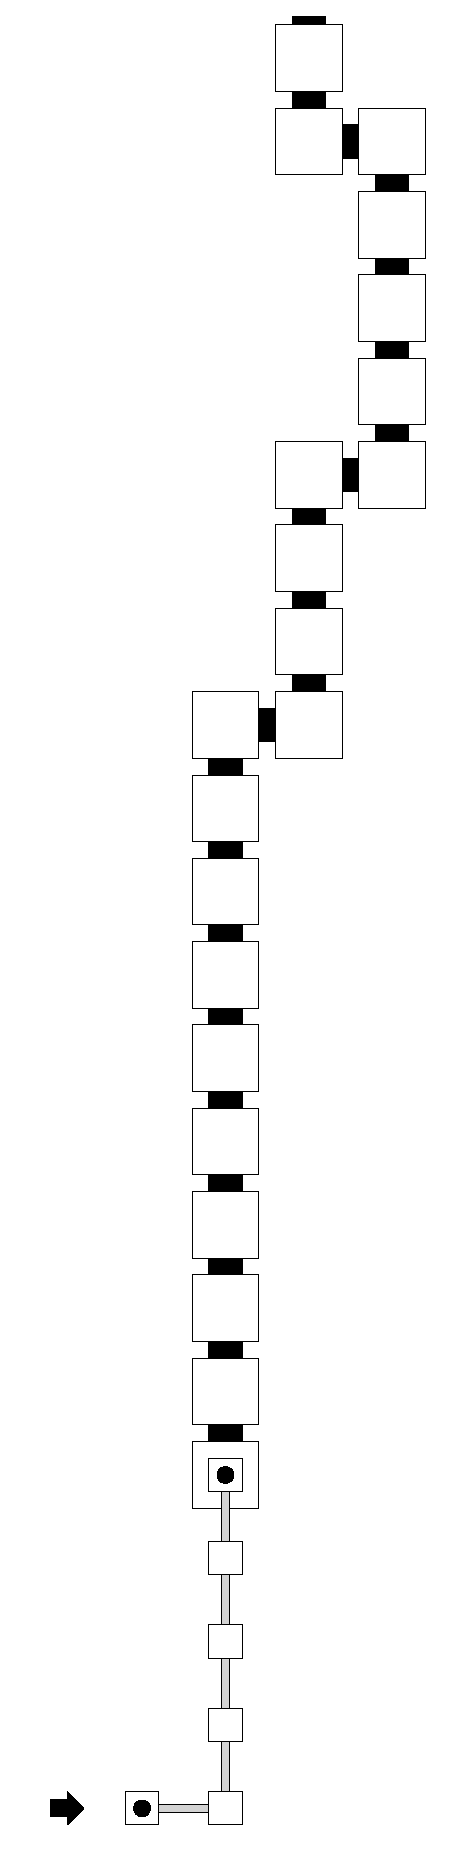
\includegraphics[width=0.17\textwidth]{warping/post_warp_general_digit1}
                \caption{\label{fig:post_warp_general_digit1} General Digit 1}
            \end{subfigure}%
            ~
            \begin{subfigure}[t]{0.17\textwidth}
                \centering
                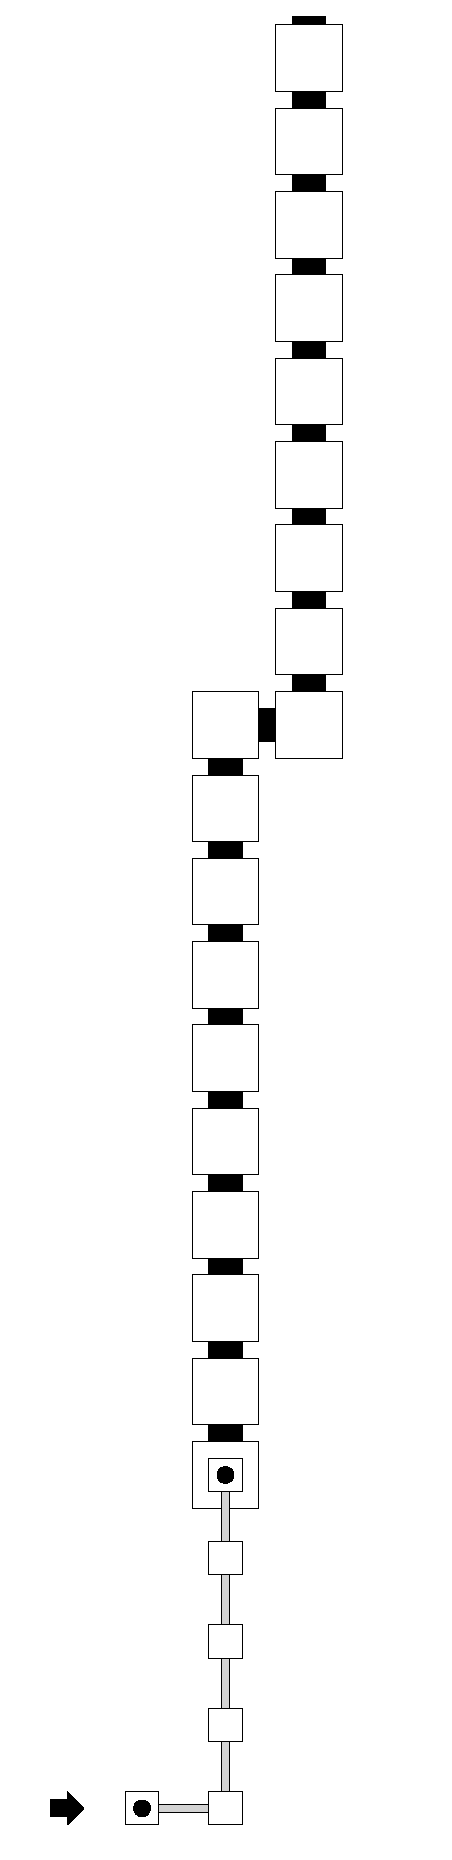
\includegraphics[width=0.17\textwidth]{warping/post_warp_general_digit2and3}
                \caption{\label{fig:post_warp_general_digit2and3} General Digits 2 and 3 }
            \end{subfigure}%
            ~
            \begin{subfigure}[t]{0.17\textwidth}
                \centering
                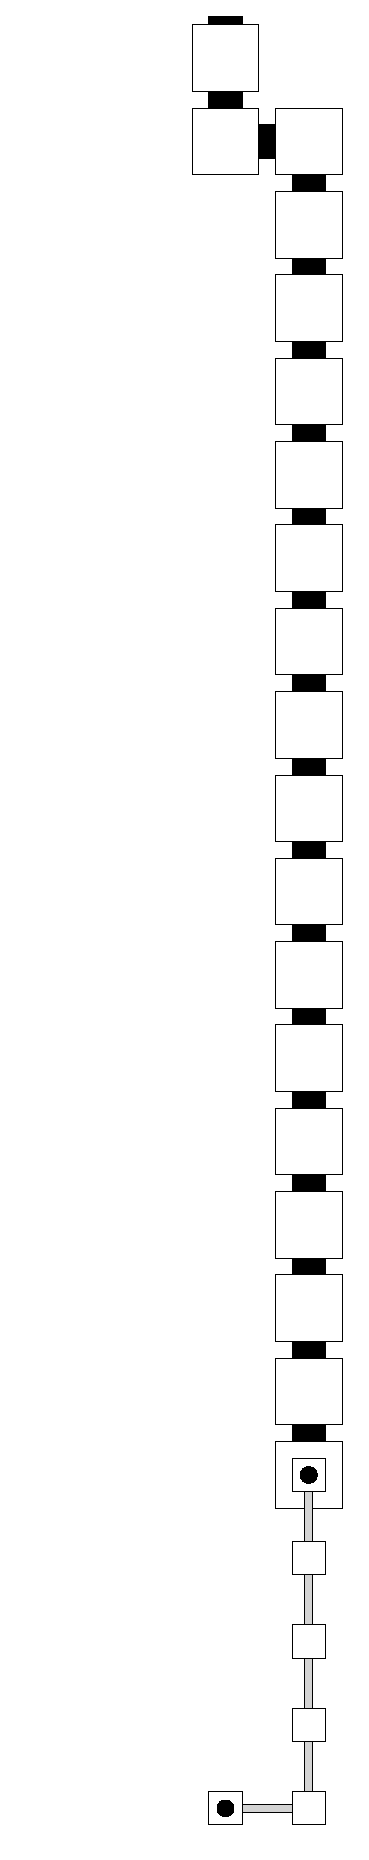
\includegraphics[width=0.17\textwidth]{warping/post_warp_case1_digit1_msr}
                \caption{\label{fig:post_warp_case1_digit1_msr} Digit 1 -- Case 1}
            \end{subfigure}%
            ~
            \begin{subfigure}[t]{0.17\textwidth}
                \centering
                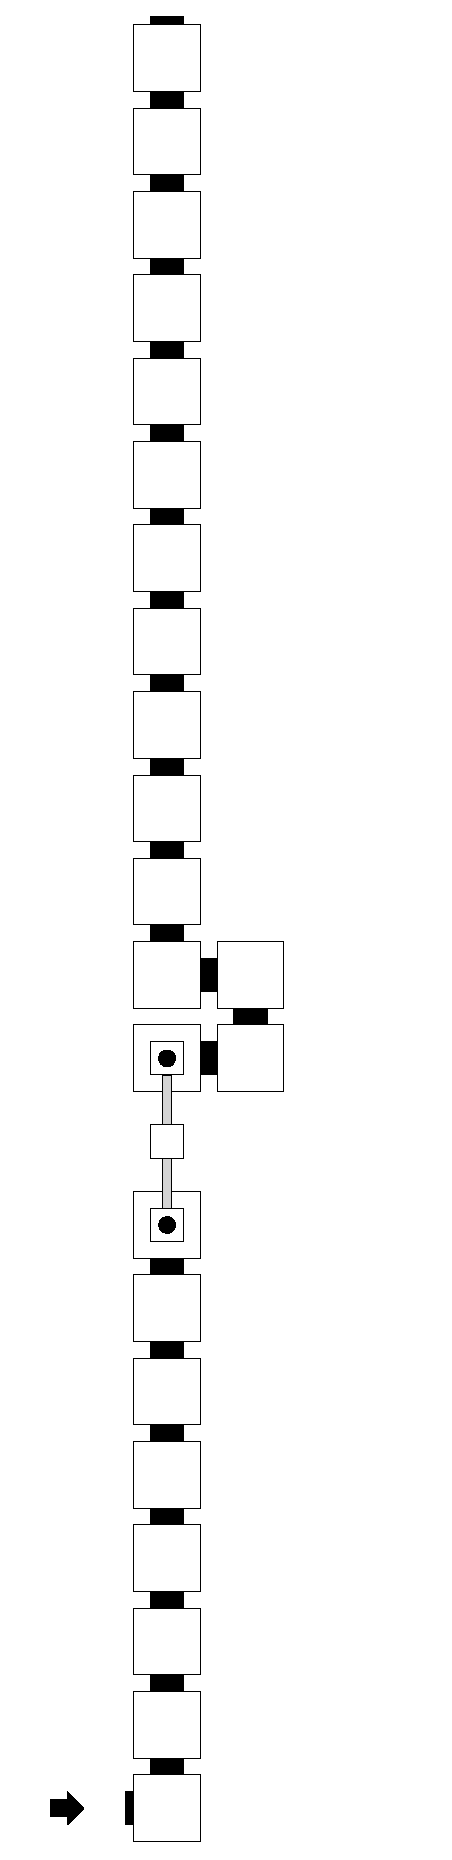
\includegraphics[width=0.17\textwidth]{warping/post_warp_case2_digit1_msr}
                \caption{\label{fig:post_warp_case2_digit1_msr} Digit 1 -- Case 2}
            \end{subfigure}%
            ~
            \begin{subfigure}[t]{0.17\textwidth}
                \centering
                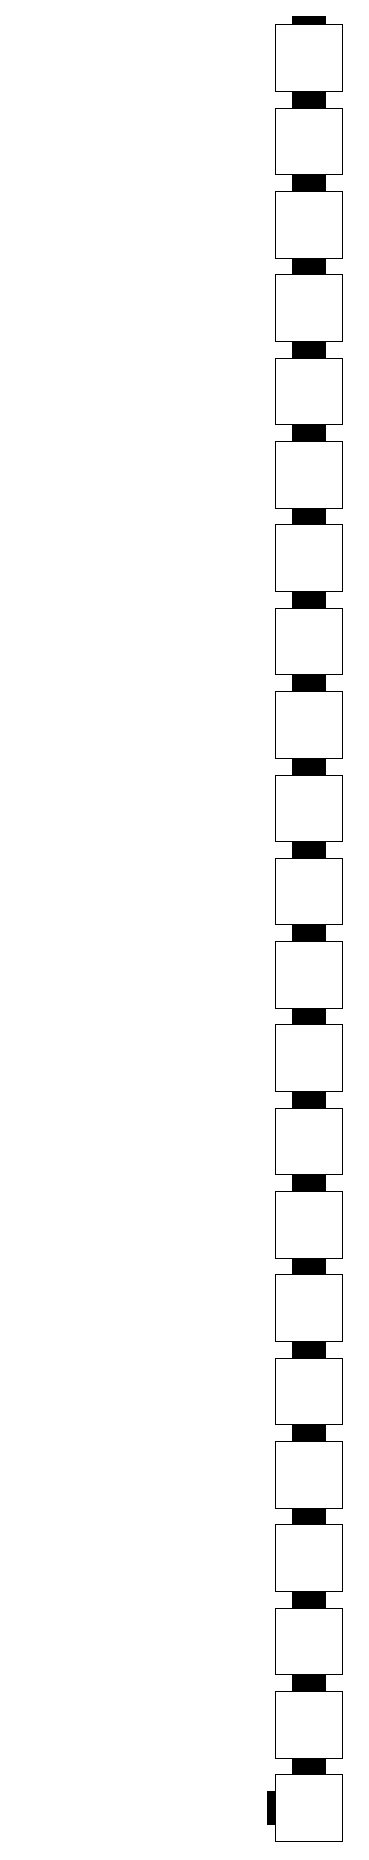
\includegraphics[width=0.17\textwidth]{warping/post_warp_case2_digit2_msr}
                \caption{\label{fig:post_warp_case2_digit2_msr} Digit 2 -- Case 2}
            \end{subfigure}%
            ~
            \caption{\label{fig:post_warp_gadgets} {\postwarp} gadgets }
        \end{figure}

    \end{itemize}
